\chapter{Wyniki i testy wydajnościowe}
\label{chap:research}

Ten rozdział zawiera zrzuty ekranu pokazujące wyrenderowane przykładowe sceny oraz testy wydajnościowe mierzące wydajność implementacji cieniowania odroczonego.


\section{Przykładowe sceny}

Używane sceny zostały przygotowane na podstawie zebranych przez Khronos w repozytorium \cite{GLTFSAMPLEMODELS} następujących przykładowych modelów glTF przedstawiających:
\begin{itemize}
	\item \textit{MetalRoughSpheres}: różne wartości metalu i chropowatości materiałów używając sfer, patrz rys. \ref{screenshot_metalroughspheres};
	\item \textit{DamagedHelmet}: uszkodzony w walce hełm sci-fi, patrz rys. \ref{screenshot_damagedhelmet};
	\item \textit{Sponza}: wnętrze budynku inspirowane pałacem Sponza, często używane do testowania oświetlenia, patrz rys. \ref{screenshot_sponza}.
\end{itemize}

\begin{figure}[!htb]
	\centering
	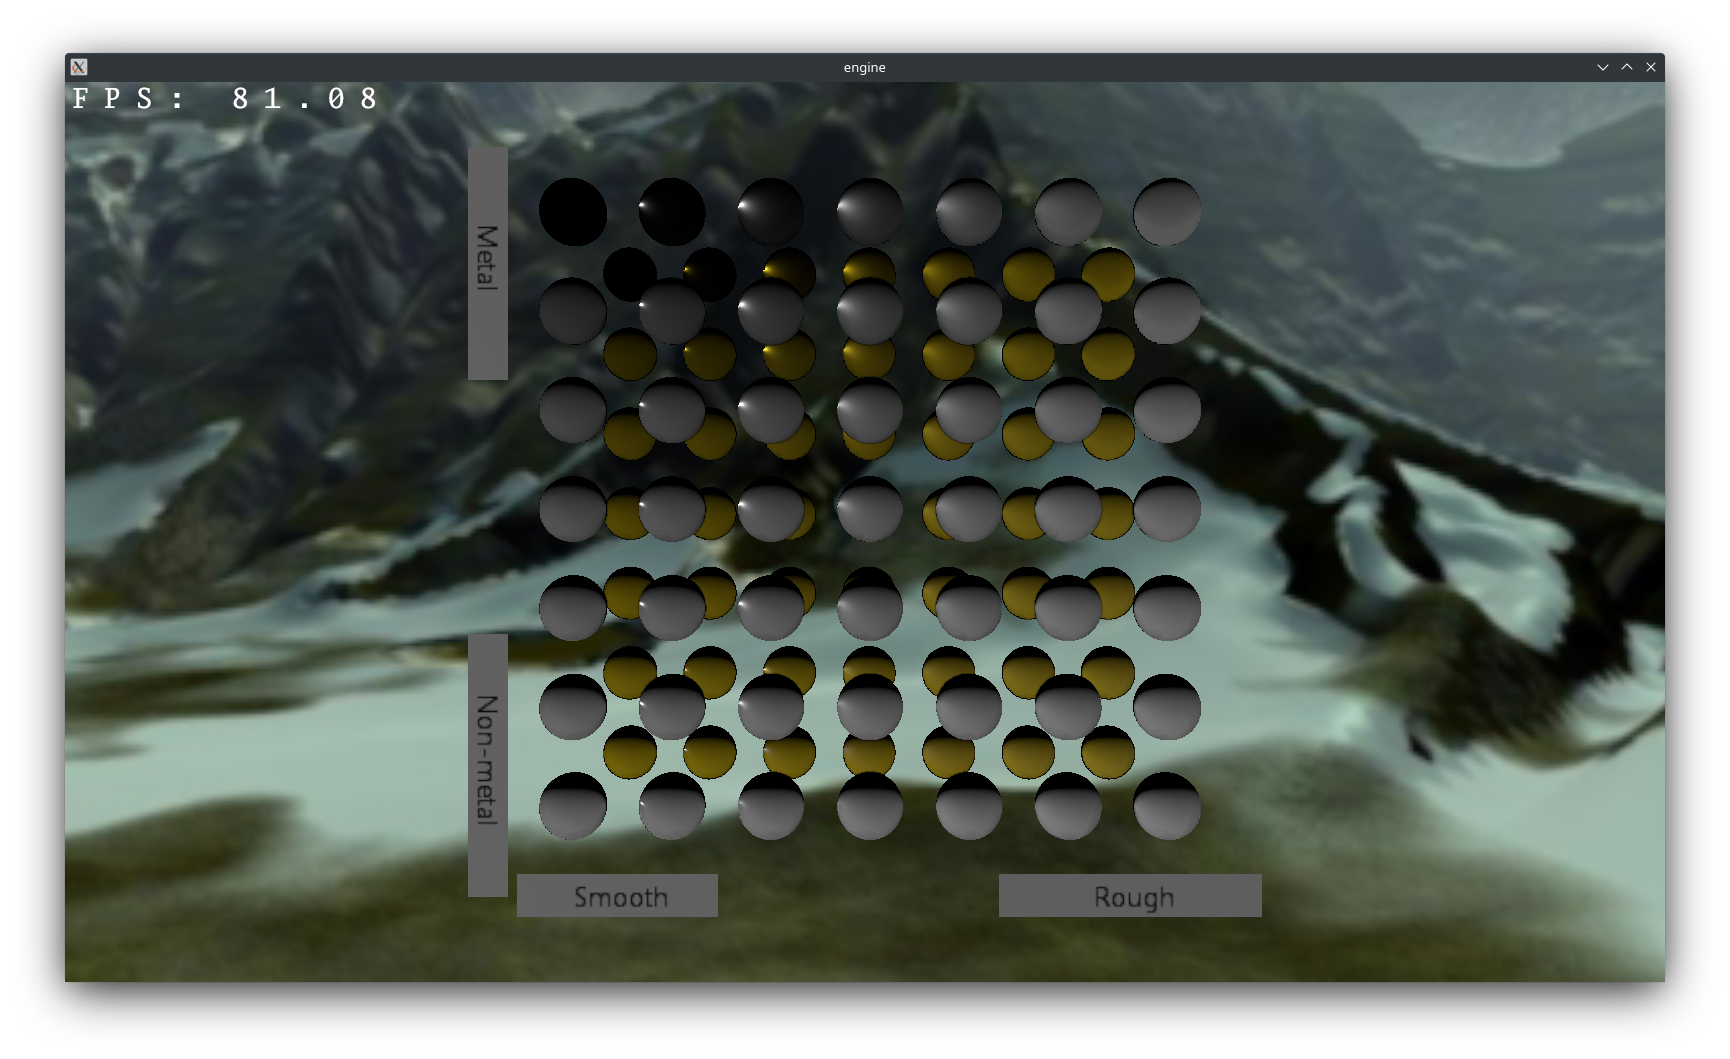
\includegraphics[width=0.8\textwidth]{images/render_metalroughspheres.png}
	\caption{Wynik renderowania sceny MetalRoughSpheres (opracowanie własne)}
	\label{screenshot_metalroughspheres}
\end{figure}

\begin{figure}[!htb]
	\centering
	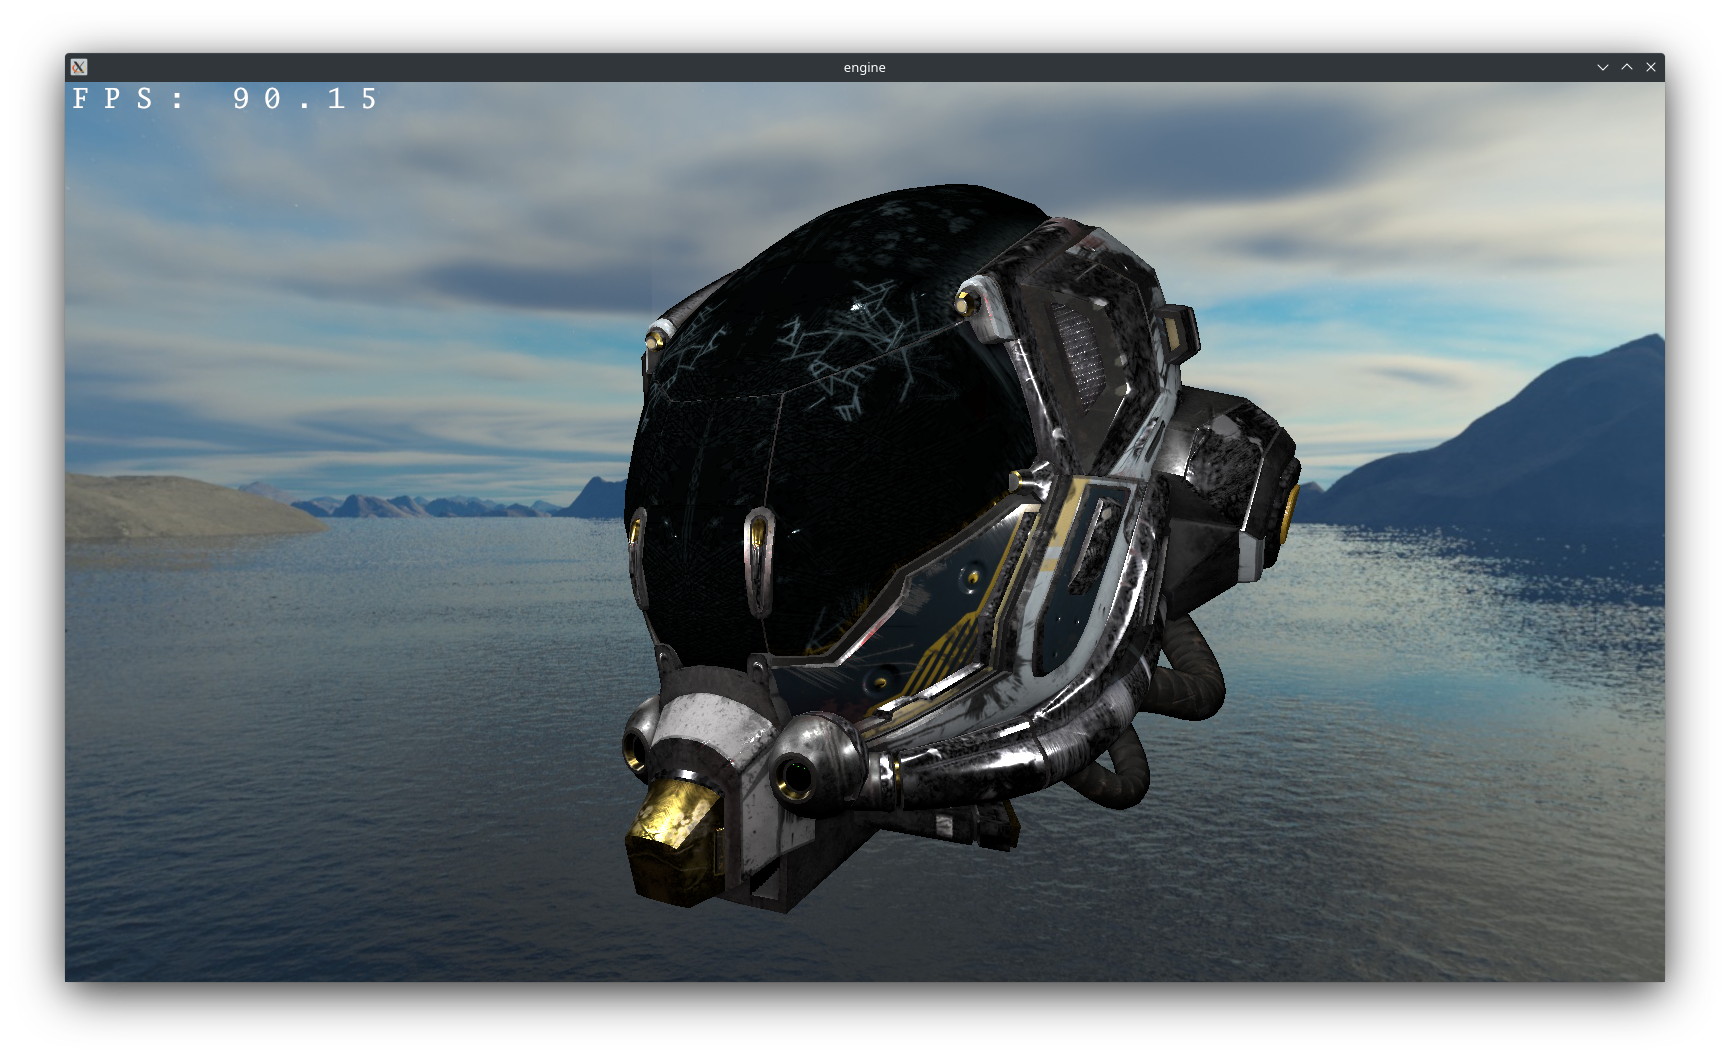
\includegraphics[width=0.8\textwidth]{images/render_damagedhelmet.png}
	\caption{Wynik renderowania sceny DamagedHelmet (opracowanie własne)}
	\label{screenshot_damagedhelmet}
\end{figure}

\begin{figure}[!htb]
	\centering
	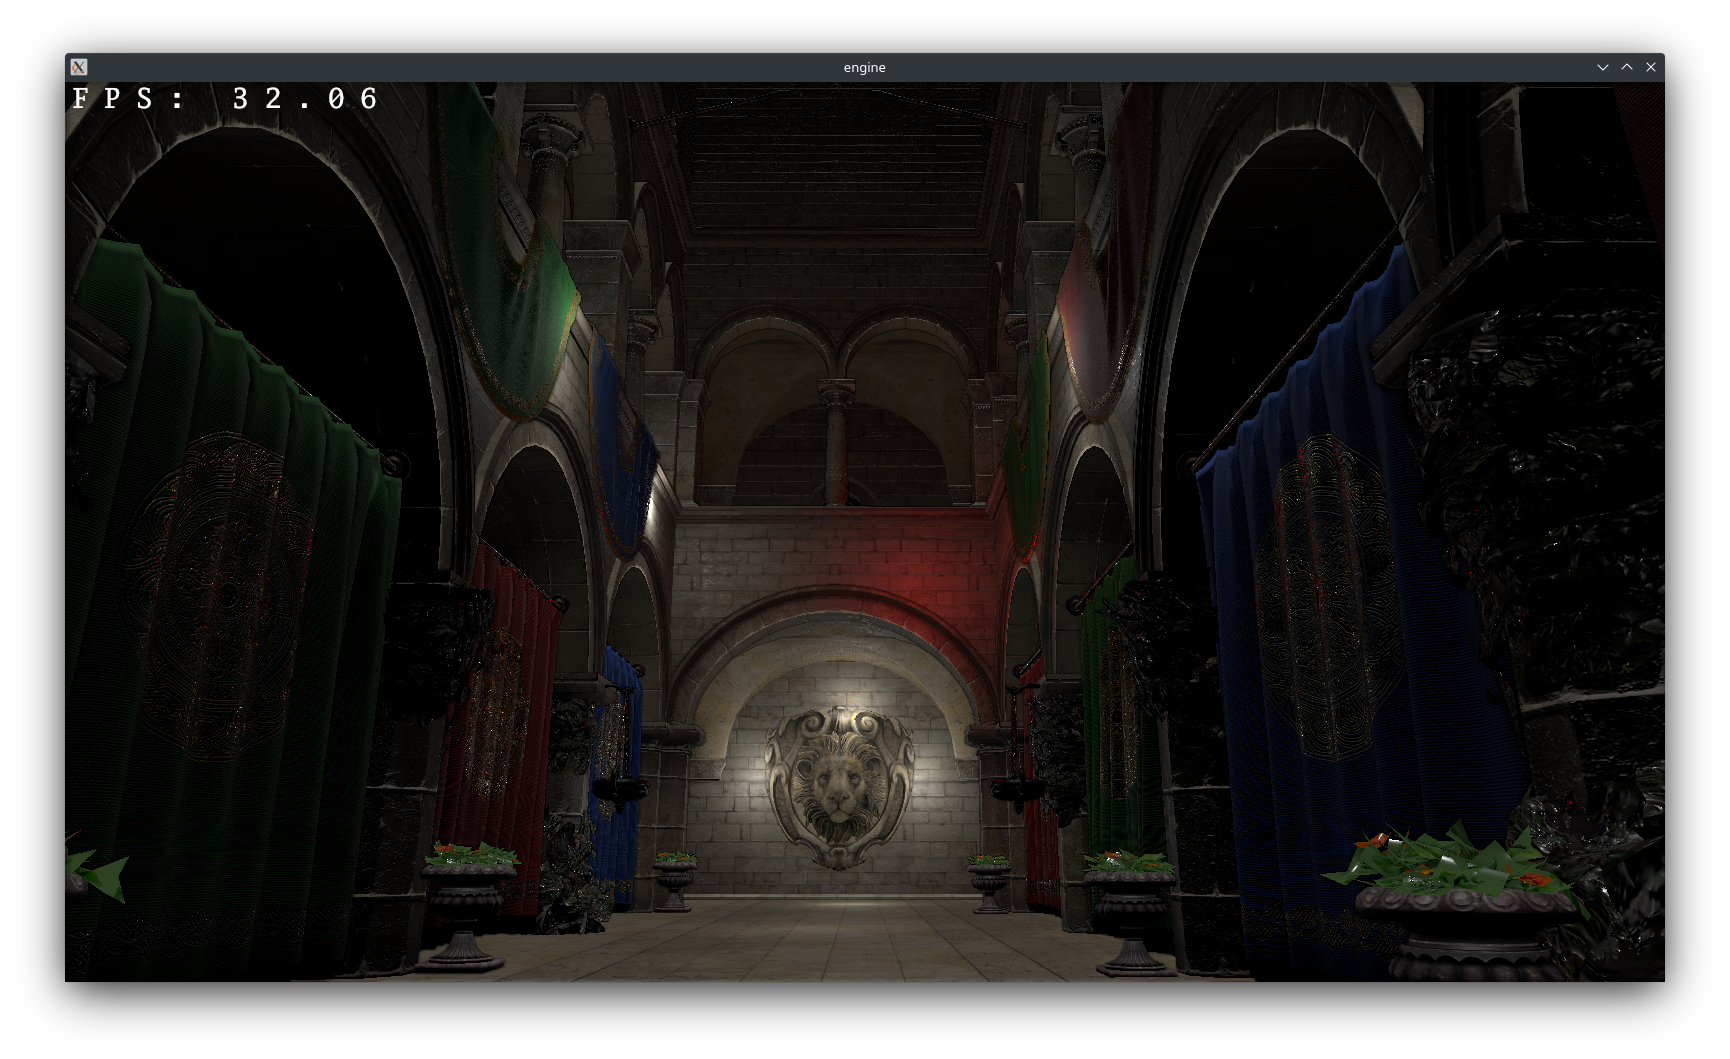
\includegraphics[width=0.8\textwidth]{images/render_sponza.png}
	\caption{Wynik renderowania sceny Sponza (opracowanie własne)}
	\label{screenshot_sponza}
\end{figure}

\section{Pomiary wydajnościowe}

Zbadano wydajność implementacji cieniowania odroczonego poprzez renderowania sceny Sponza w 10 eksperymentach spowodowanych zmianą następujących zmiennych:
\begin{itemize}
	\item rozdzielczości okna: 640x480, 1600x900;
	\item liczby świateł punktowych: 1, 30, 75, 10, 100.
\end{itemize}

Zmierzono liczbę klatek na sekundę poprzez obserwację maksymalnych i minimalnych wartości wyświetlanych podczas działania programu licznik FPS silnika w lewym górnym rogu okna, które są zbliżone do wartości reportowanych przez warstwę \textit{VK\_LAYER\_MESA\_overlay}.

Zmierzono udział poszczególnych etapów potoku graficznego podczas wykonywania poleceń rysowania poprzez przechwycenie 10 klatki aplikacji narzędziem RenderDoc i zbadanie liczników wydajności.
Po porównianiu wartości liczników wydajności z przechwyconych klatek okazało się, że największe zmierzone zmiany, które nie mogą być wytłumaczone błędem przypadkowym spowodowanym nieprzewidywalnością działania potoku graficznego GPU, zachodzą tylko dla liczników wydajności najdłużej wykonującego się polecenia rysowania w przebiegu oświetlenia G-bufora:
W pomiarach zostały uzględnione poniższe liczniki:
\begin{itemize}
	\item \textit{GPU Time Elapsed ($\mu$)}: czas jaki upłynął na GPU podczas wykonywania polecenia;
	\item \textit{L3 Shader Throughput (bytes)}: całkowita liczba bajtów pamięci GPU przesyłanych pomiędzy shaderami a pamięcią podręczną L3;
	\item \textit{Shader Memory Accesses}: całkowita liczba operacji dostępu do pamięci buforów w shaderach;
	\item \textit{Sampler Texels}: całkowita liczba tekseli widocznych na wejściu wszystkich próbników (z dokładnością 2x2),
	\item \textit{Samplers Busy (\%)}: procent czasu spędzony na próbkowaniu obrazów.
\end{itemize}
Wartości wszystkich zmierzonych liczników mają stałą wartość z wyjątkiem \textit{GPU Time Elapsed ($\mu$)} i \textit{Samplers Busy (\%)} obarczonych błędem przypadkowym.

Wyniki pomiarów wydajności prezentuje tabela \ref{results_sponza}.
// HIRO FPS Avg
\begin{table}[!ht]
	\centering
	\begin{tabular}{ |p{2cm}|p{1.1cm}||p{0.6cm}|p{0.6cm}||p{1.7cm}|p{1.8cm}|p{1.5cm}|p{1.3cm}|p{1.3cm}|}
		\hline
		Rozdzielczość okna & Liczba świateł & FPS Min & FPS Max & GPU Time Elapsed ($\mu$) & L3 Shader Throughput (bytes) & Shader Memory Accesses & Sampler Texels & Samplers Busy (\%) \\
		\hline \hline
		640x480 & 1 & 101 & 129 & 1859.916 & 19685376 & 307584 & 1228800 & 97.3006 \\
		\hline 
		640x480 & 10 & 86 & 104 & 7457.666 & 68837824 & 1075591 & 1228800 & 88.82873 \\
		\hline 
		640x480 & 30 & 70 & 79  & 7299.75 & 179433088 & 2803642 & 1228800 & 50.89936 \\
		\hline 
		640x480 & 75 & 46 & 48 & 37235.50 & 428882496 & 6701289 & 1228800 & 26.02086 \\
		\hline 
		640x480 & 100 & 37  & 40 & 23358.666 & 566511168 & 8851737 & 1228800 & 20.69141 \\
		\hline 	\hline 
		1600x900 & 1 & 37  & 42 & 3819.166 & 92281664 & 1441901 & 5760000 & 99.45081 \\
		\hline 
		1600x900 & 10 & 29  & 31 & 14263.333 & 322695168 & 5042112 & 5760000 & 89.91253 \\
		\hline 
		1600x900 & 30 & 19 & 21 & 34444.083 & 841100544 & 13142196 & 5760000 & 57.64096 \\
		\hline 
		1600x900 & 75 & 11 & 12 & 82389.333 & 2010387968 & 31412312 & 5760000 & 26.82165 \\
		\hline 
		1600x900 & 100 & 9  & 10 & 109205.75 & 2655508160 & 41492315 & 5760000 & 21.54303 \\
		\hline
	\end{tabular}
	\caption{Wyniki pomiarów dla sceny Sponza (opracowanie własne)} 
	\label{results_sponza}
\end{table}


\section{Analiza pomiarów}

Działanie renderera spowalnia wraz z zwiększającą się liczbą świateł oraz rozdzielczością okna.

Spowolnienie spowodowane zmianią rozdzielczości może być wytłumaczone zmianą wielkości G-bufora i tym samym zwiększeniem liczby wykonywanych shaderów fragmentów.

Zwiększenie liczby świateł zwiększa liczbę obiegów pętli w przebiegu oświetlania pobierających informacje o każdym świetle z bufora uniform, co tłumaczy rosnącą liczbę dostępów do pamięci i malejący udział procentowy czasu spędzonego na próbkowaniu G-bufora.

// HIRO analizę pomiarów dobrze byłoby trochę rozbudować
